%-------------------------------------------------------------------
% bachelor thesis
% create by: Mario Preishuber
% create date: 2014, Jan 01.
%-------------------------------------------------------------------

\section{Mutator Heap Analysis} \label{sec:analysis_mutator}

In this section we describe how to some interesting heap properties and present our analysis results of the mutator heap. For our analysis we only care about object types which can be allocated by a mutator. These object types are arrays, strings, user-defined objects, code, closures, regular expressions (regexp), and numbers. We analyzed the distribution of object types, sizes and lifetimes, the number of outgoing edges, and the distance from the GC roots to the objects. 
The type information is part of a heap snapshot. The distribution of object types is computed over all workloads, i.e., all snapshots of all real-world application. Figure \ref{fig:obj_alloc_dist} presents the distribution of object types as a histogram. A heap snapshot contains not only objects with a type presented in the histogram. There are several V8 specific types like hidden classes which describe a internal representation of object properties, and GC roots have the type synthetic. We do not care about the V8 specific types, to be platform independent. Our analysis show that the most objects are of type array, string, or user-defined object. The dominance of arrays differs from the results in \cite{JSMeter2009}. A reason for this behavior is if it is necessary to a copy an array because it grows too much, we treat the new array logically as a new heap object. This behavior results in an increasing number of objects and the average lifetime decreases. 
\begin{figure}
	\centering
	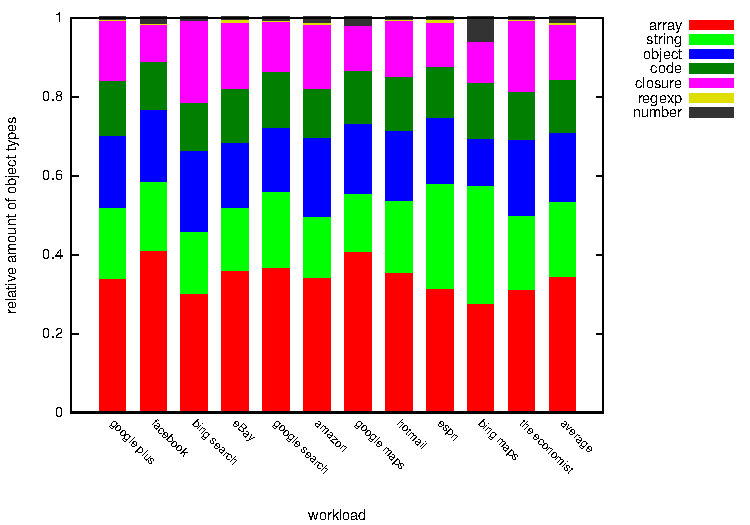
\includegraphics[width=0.5\textwidth]{obj_alloc_dist}
	\caption{Histogram of the object type distribution for all workloads, confirms \cite{JSMeter2009}.}
	\label{fig:obj_alloc_dist}
\end{figure}

Figure \ref{fig:obj_selfsize_dist} shows the object size distribution for each type. The x-axis displays the object size in byte and the y-axis shows the relative amount of objects living shorter than x. Each object on the \JS heap is identified by a unique V8 internal id which is a property of a heap snapshot. The size of a object is also a property of a snapshot. This allows us to count objects of the same size of all snapshots of all workloads. As the figure shows depends the object size distribution on the type of the objects. There are a few large object and a lot of small objects. This behavior is similar to the allocation behavior of C programs which is shown in \cite{Aigner2013}. The figure also shows that there are object types with a fix size, e.g., numbers with a size of 12 byte.
\begin{figure}
	\centering
	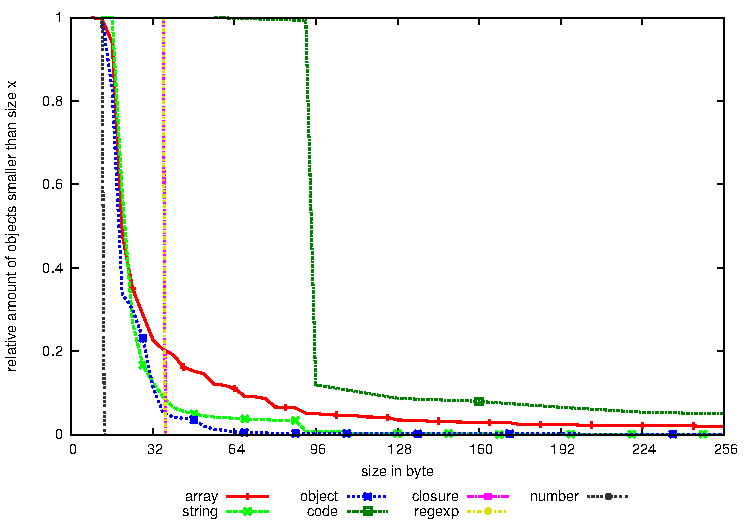
\includegraphics[width=0.5\textwidth]{obj_selfsize_dist}
	\caption{Size distribution of real web applications, confirms \cite{JSMeter2009}.}
	\label{fig:obj_selfsize_dist}
\end{figure}

As explained above it is possible to identify an object by an unique id which never changes. This fact allows us to compute the lifetime of an object. Figure \ref{fig:obj_lifetime_dist} illustrates the distribution of the lifetime of all snapshots of all workloads separated by the object type. The lifetime is measured in allocated bytes which are allocated during a object is live. As a result of the sampling rate of the snapshot generation which is 4 KB, the minimum lifetime of a object is also 4 KB. These amount of allocated byte is displayed on the x-axis and on the y-axis is the relative amount of objects living shorter than x presented. The figure shows that the lifetime of arrays is significant smaller the lifetime of strings. What results of the fact, if a array has to be copied, because of growing too much, a logically new array is created. This approach influences the liveness of arrays, but from the garbage collector perspective this way of counting is okay, because the old array also has to be deallocated.
\begin{figure}
	\centering
	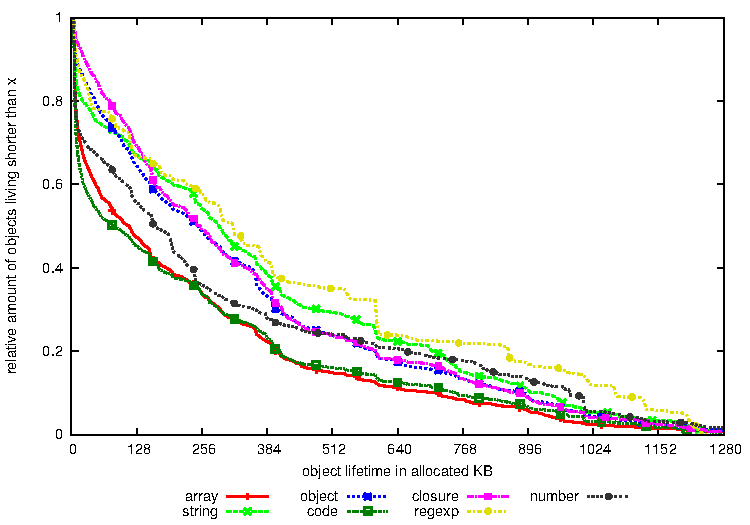
\includegraphics[width=0.5\textwidth]{obj_lifetime_dist}
	\caption{Lifetime distribution of real web applications, confirms \cite{JSMeter2009}.}
	\label{fig:obj_lifetime_dist}
\end{figure}

An important property of a heap structure is the depth of a heap graph. So we computed the minimum distance of a node to it's GC root. A heap snapshot contains special nodes which represent GC roots, these nodes are of the type synthetic. We use a recursive depth-first search algorithm and compute the root distance for each node of all snapshots of all workloads and separated again by type. The x-axis of Figure \ref{fig:obj_rootdist_dist} shows the minimum root distance and the y-axis presents the relative amount of objects with a root distance smaller than x. This figure shows that the most objects have a small root distance.
\begin{figure}
	\centering
	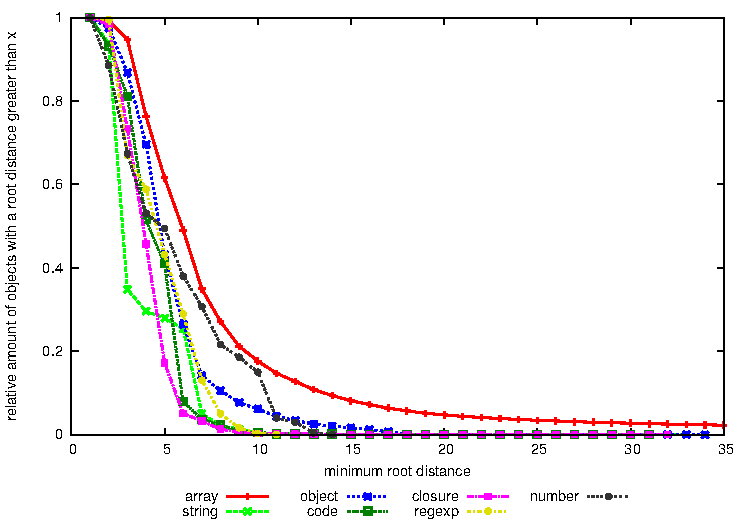
\includegraphics[width=0.5\textwidth]{obj_rootdist_dist}
	\caption{GC root distance distribution of real web applications, confirms \cite{JSMeter2009}.}
	\label{fig:obj_rootdist_dist}
\end{figure}

Another interesting property by talking about the structure of a heap is the number of outgoing edges of a node. The number of outgoing edges, the so-called out-degree, results of the fact that the snapshots represent a directed graph. So this information is provided by the heap snapshots. Figure \ref{fig:obj_outdeg_dist} shows the distribution of the out-degree separated by the object type. The out-degree is computed for each node of each snapshot of all workloads. The x-axis of the figure presents the out-degree and on the y-axis is the relative amount of objects with an out-degree smaller than x displayed. Arrays have a low out-degree what indicates that most arrays contain primitive types. 
\begin{figure}
	\centering
	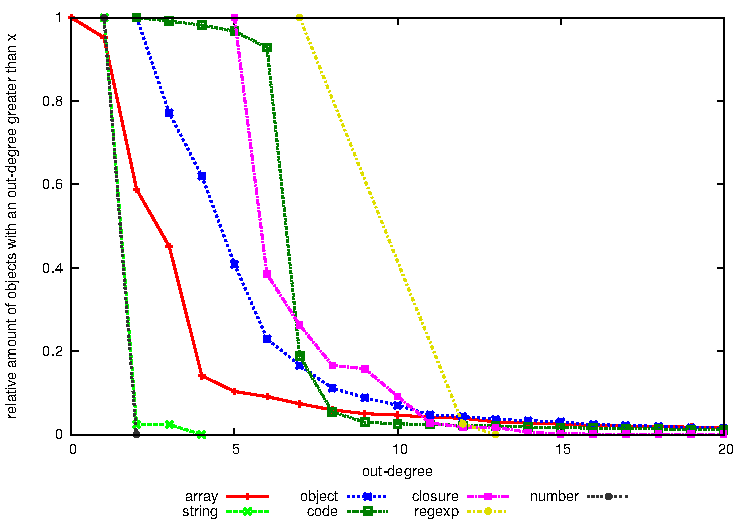
\includegraphics[width=0.5\textwidth]{obj_outdeg_dist}
	\caption{Out-degree distribution of real web applications, confirms \cite{JSMeter2009}.}
	\label{fig:obj_outdeg_dist}
\end{figure}

If we talk about the out going edges of a node we want also to know how the number of in-going edges looks like. The number of in-going edges, the so-called in-degree, is not an explicit property of a snapshot, i.e., it requires some computations. In other words the in-degree represents the number of parents a node has and this is the way how it is computed. Before inserting a snapshot into the database some preparations are required and during these preparations the number of parents of a node is counted. Figure \ref{fig:obj_indeg_dist} shows the distribution of the in-degree over all nodes of all snapshots of all workloads separated by type. On the x-axis is the in-degree displayed and on the y-axis is the relative amount of objects with an in-degree smaller than x is shown. The figure presents a quite different behavior than Figure \ref{fig:obj_outdeg_dist} which shows the out-degree distribution. The behavior of the different types is more similar that it is for the out-degree. As expected have strings a higher in-degree, because often are strings allocated once and reused.
\begin{figure}
	\centering
	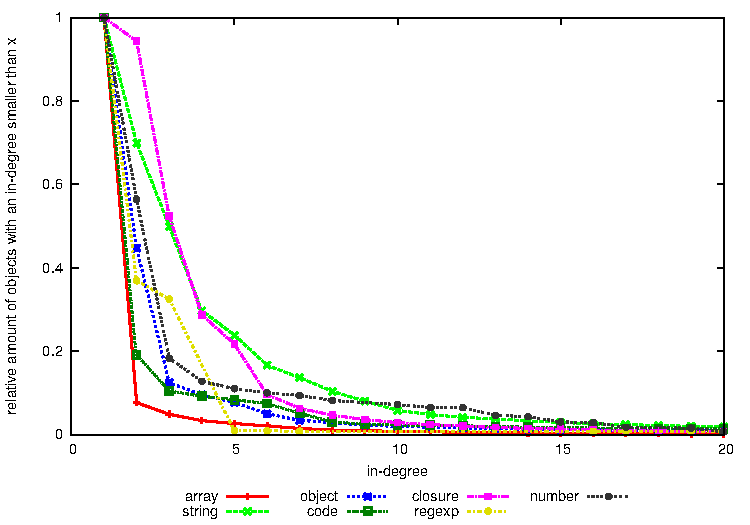
\includegraphics[width=0.5\textwidth]{obj_indeg_dist}
	\caption{In-degree distribution of real web applications, confirms \cite{JSMeter2009}.}
	\label{fig:obj_indeg_dist}
\end{figure}

To complete our analysis of the heap structure we have a look at strongly connected components. We compute the strongly connected components with the Trajan's algorithm \cite{Trajan}. We are interested in the size of a strongly connected component, i.e., the number of edges which the components contains. What we also want to know is the number of strongly connected components of a heap graph. One snapshot represents the current heap, since a heap is a directed graph we analyzed each snapshot separate. The Table \ref{tab:scc_stats} shows our analysis results, the values are the average values of all snapshots of all workloads. If we compare the average and the median of the quantity we recognize a significant difference. This comparison shows there are some extreme values, which is also illustrated by the maximum, but the most heaps contain less then 50 strongly connected components. The size of these strongly connected components presents a similar result. There are a lot of small strongly connected components and a few large.
\begin{table}
	\small
	\centering
	\begin{tabular}{l r r}
		\toprule
		\textbf{strongly connected components} & \textbf{size} & \textbf{quantity} \\ \midrule
		minimum							&	0.286		&	0.782			\\ 
		maximum							&	53,729.857	&	285.916			\\ 
		average							&	5,316.409	&	11.177			\\ 
		quantile 25						&	2,304.786	&	3.107			\\ 
		quantile 50						&	3,082.429	&	6.329			\\ 
		quantile 75						&	3,629.714	&	14.655			\\ 
		quantile 90						&	12,199.429	&	36.211			\\ 
		quantile 95						&	25,979.000	&	49.448			\\ \bottomrule
	\end{tabular}
	\caption{Summary of the measurements of strongly connected components.}
	\label{tab:scc_stats}
\end{table}